In the following chapter the current creation and signing process of quotations and order confirmation for customer projects are described.

There is no existing \gls{cms} at the moment. \Gls{cc} has a process established that fulfills partly the signing guideline of the company. In the appendix \ref{bpmnOld} the business process from the initial state is visualized. The process will be described the section \ref{sec:bp}.

\section{Signing Guideline} \label{sec:signingGuideline}

\Gls{cc} has a signing guideline, which is for the thesis summarized in table \ref{tab:summarySignatureGuideline}:
\begin{table}[h!]
	\begin{tabular}{|p{3cm}|p{2cm}|p{10cm}|}\hline
		\rowcolor{Gray}Position & Amendment & Document Types \\ \hline
		Chairman & - & All document types can be signed. \\ \hline
		Procurator & ppa & All employees belonging to this group have the right to sign all documents with the same rights as the chairman.\\ \hline
		Site \& \gls{hr} manager & i.V. & The group has a general authority to sign documents, but there are more exceptions, where they need to sign together with one from the governing board or the procurator. One important point is that the project contract and partner quotation with an amount less than 50.000 \euro can be signed without them, everything above need to be signed together with them. There a more exceptions, but they are only for specific cases, that will be explained below. \\ \hline
		All other employees & i.A. & This group is allowed to create quotations and sign them if this belongs to their tasks and the amount of the quotation is not higher than 50.000 \euro. \\ \hline
	\end{tabular}
	\caption{Summary Signature Guideline of codecentric AG}
	\label{tab:summarySignatureGuideline}
\end{table}

The exceptions for the site and \gls{hr} managers are the following: all topics regarding the area loan and dept, lease contracts, buying and sale of cars, every type of contract that needs the handwritten signature and juristic acts.

The guideline defines strict regulations. Important is that there are some conditions regarding the type of document and the price of a contract or quotation. This needs to be known by the person who wants to sign a document. Additional information about the positions of employees is required.

\section{Business Process} \label{sec:bp}
First of all the used terminologies and involved user groups of the business process are explained, next the general process is briefly described followed by the relevant subprocesses.

\subsection*{Terminologies}
At \gls{cc} different terminologies are used, which are also used to explain the business process. To get an understanding of them they are listed here:
\begin{itemize}
	\item Quotation: \newline
	Is a document in which \gls{cc} gives the customer an overview about the approximated work, necessary software, hardware and costs to their requested project. This document type is divided in two subcategories. This is important to distinguish between them, because the creation of them is different. In the following they will be explained:
	\begin{enumerate}
		\item Simple Quotation: \newline
		An uncomplicated quotation, which has only a few listings of needed Software and Hardware and estimated working time and their prices. It is always based on the \gls{gtct}.
		\item Complex Quotation: \newline
		A quotation for a bigger project or company. Inside this document a lot of explanations about tasks and topics are placed. Also, the amount is mostly higher than 50.000 \euro and can have regulations regarding the paying of the amount. Furthermore, this type may be have different legal foundation than a simple quotation. Moreover, it could be that inside this project external employees are involved and the quotation explains the conditions of this situation. In general with this quotation type more interactions with the customer is required. 
	\end{enumerate}
	\item Order: \newline
	A document send from the customer to \gls{cc}, that has as content the information which quotation is accepted. Furthermore, it needs to be signed by the customer.
	\item Order Confirmation: \newline
	This document is sent from \gls{cc} to the customer with the information that the order is accepted and will be processed by a team of \gls{cc}.
\end{itemize}
\newpage
\subsection*{Involved User Groups}
Currently the following parties are involved in the business process: 
\begin{table}[h]
	\begin{tabular}{|p{0.25cm}|p{2cm}|p{13cm}|} \hline
		\rowcolor{Gray}\# & Role & Description \\ \hline
		1 & Customer & This user group wants to have a product/solution for a problem. In this process the aim is to get a project or order from the customer. So he needs to be satisfied. \\ \hline
		2 & Sales & This user group creates the quotations and will process the orders if the quotations are accepted by the customer. \\ \hline
		3 & Backoffice & This actor group coordinates the incoming orders and keeps track of the completeness for all documents needed for the order. \\ \hline
		4 & Executive Board & Consists out of chairmans and procurators of \gls{cc}. This group is only involved inside the process if the amount of a quotation is higher than a defined amount (defined in the signing guideline). Then one of them need to sign/agree on the document. \\ \hline
	\end{tabular}
	\caption{Roles Involved in the Old Business Process}
	\label{tab:bpRoles}
\end{table}

\subsection*{General Process}
The general process is visualized in figure \ref{fig:0_main}. Mainly involved are the sales and the backoffice department. The only interaction with the customer is to exchange documents and information, which are needed to create the documents for the possible projects. There is also a clear division of tasks. The Sales is responsible for the quotations and the backoffice for coordinating and setting up the requirements to start working on the orders coming in based on the quotations.

\begin{figure}[h!]
	\begin{center}
		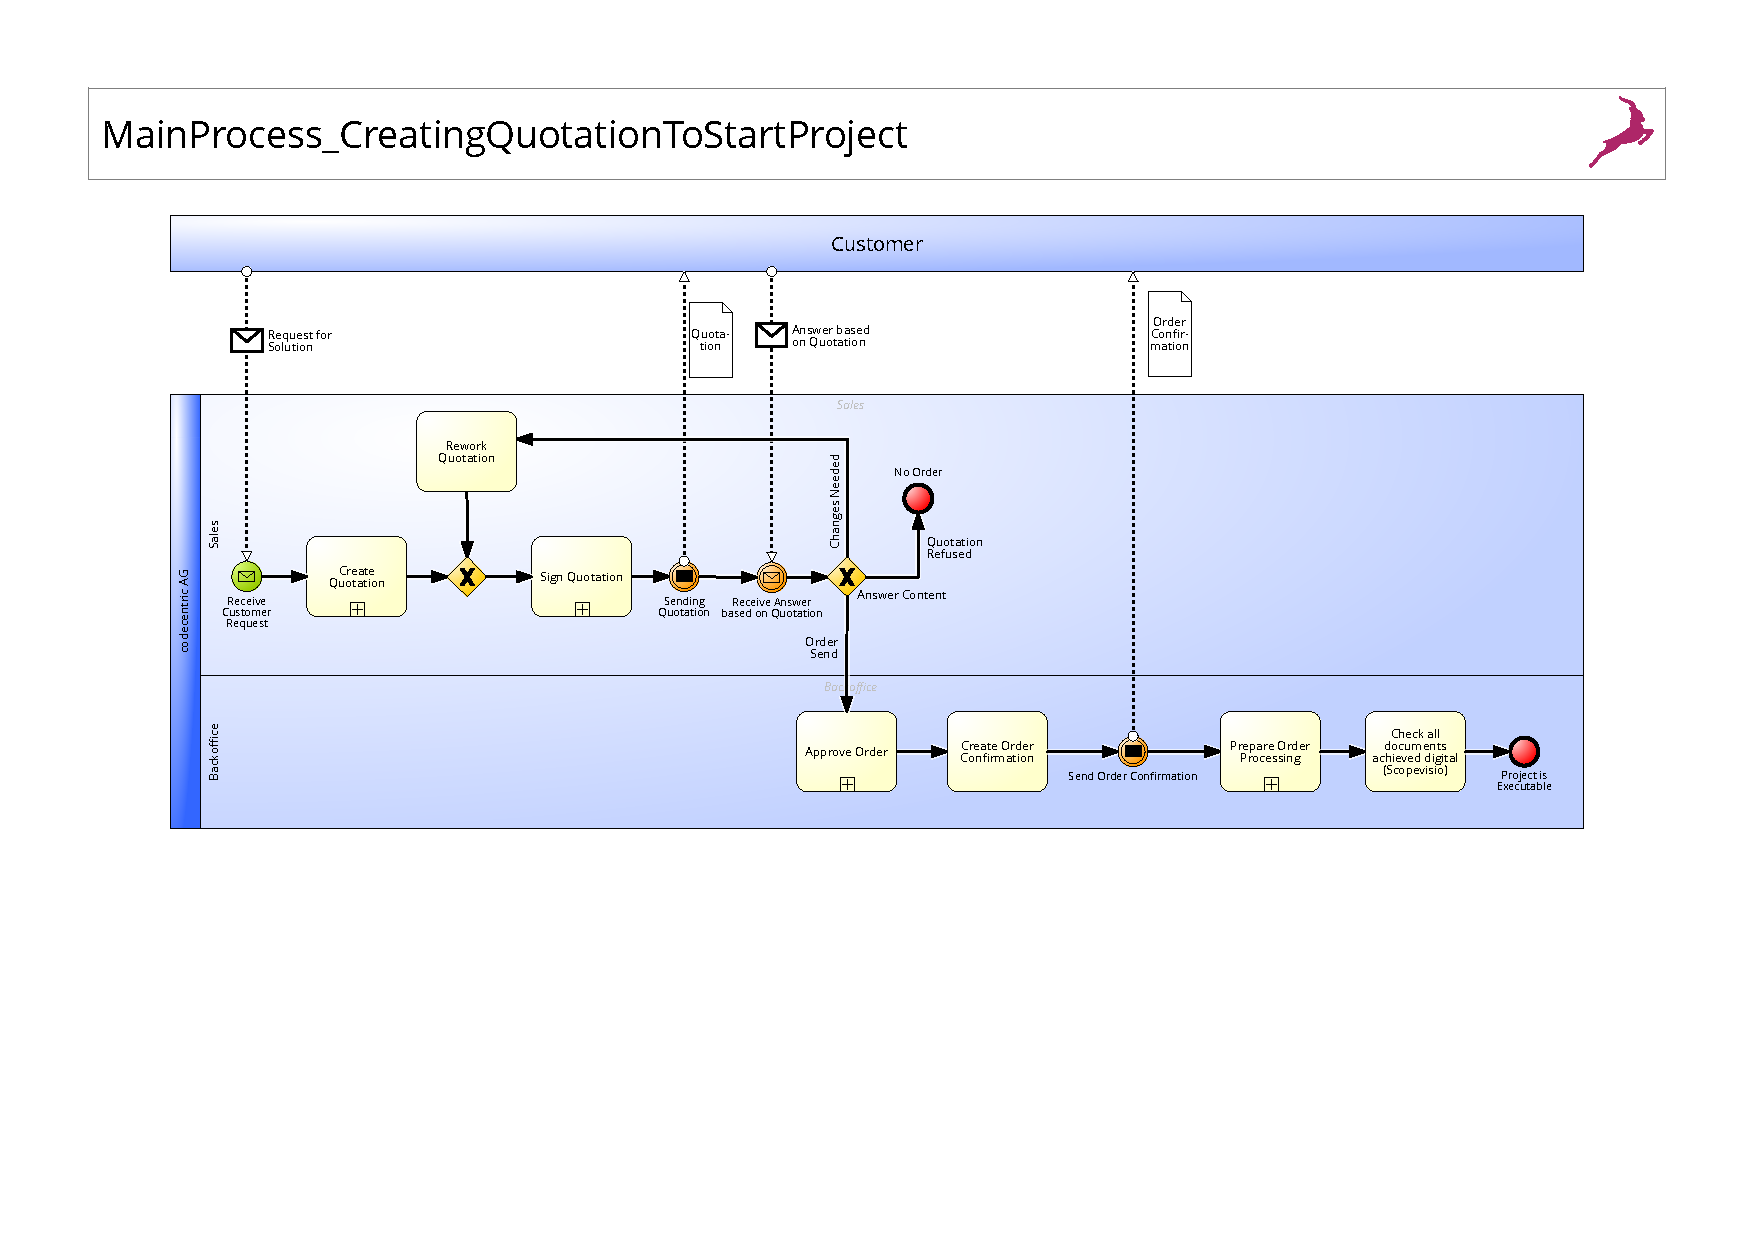
\includegraphics[width=\textheight,angle=90]{./appendix/pbmnOld/0_main.pdf}
		\caption{Main Old Process}\label{fig:0_main}
	\end{center}
\end{figure} 

The used technologies and tools in this process are mainly the current \gls{erp} \textit{Scopevisio}, \textit{Microsoft Word} and \textit{Google Docs}, sometimes \textit{DocuSign} is also used. With the first one the basic information of the document is created and maintained, the simple quotations are generated out of it and all documents are stored based on a defined structure. With \textit{Microsoft Word} and \textit{Google Docs} mostly the more complex quotations and the contracts are created. The employees can choose which one of the two tools they will use. \textit{DocuSign} is an online tool that provides functionality to sign documents electronically.

\subsection*{Subprocesses}
In the general process several subprocesses are mentioned. Each of them will be described.

The first subprocess is the creation of the quotation visualized in figure \ref{fig:0-1_sub}. This process is placed in the sales department. They use the \gls{erp} tool \textit{Scopevisio} to generate the metadata of the quotation and depending on the category of the possible project either a simple quotation is generated or a complex quotation.

In the figure \ref{fig:0-2_sub} the second subprocess is shown. It visualizes the signing process of a quotation. The document needs to be signed regarding the signing guideline of \gls{cc}. An overview is given in section \ref{sec:signingGuideline}. At a certain price level the executive board needs to sign the contract additionally. At the moment the signing can be done in two ways. First manually on paper and afterwards send the contract in duplicate to the customer with a letter. Or scanned the signed contract and then send it by email to the customer. Sometimes it happens that the signing is ignored by the employees.

The next subprocess is the approval of the order of the customer, presented in figure \ref{fig:0-3_sub}. The backoffice checks if the order is conform to the stored quotation in \textit{Scopevisio}. In the case there are some inconsistencies they will be removed. Finally, the order is approved.

The last subprocess is the setup of the order processing. This process is presented through the figure \ref{fig:0-4_sub}. First the backoffice informs the project manager that they successfully agreed with the customer. At this point the next subprocess is started. This is shown in figure \ref{fig:0-4-1_subsub}. In the case that additional licenses or hardware components are required, they will be ordered and the invoices and delivery tickets will be added to \textit{Scopevisio}. Then it goes back to the previous process. \newline
The backoffice identifies the persons, that should process the order, and is creating for them a task ticket on \textit{Jira}, a tool for tracking projects and their progress. In the case that the employees are unknown, the project manager is requested to determinate them. Next all involved employees get the information about the ticket and the processing of the order can be started.

\section{Issues \& Problems} \label{sec:issues}
At the moment there are several issues and problems with the process. The major problem is that most documents are signed manually. This leads to several other problems:
\begin{itemize}
	\item The signing process can take a lot of time: \newline
	Due to the fact that some document types need to be signed from one of the governing board, leads this to a further problem: There are fourteen sites without a person having this status, the document needs to be sent to the headquarter of \gls{cc} in Solingen. Therefore, three options exist:
	\begin{enumerate}
		\item Sign the document, scan it afterwards and send it via email to the headquarter and back to the site, which makes a lot of effort and manual actions.
		\item Sign the document and send it with a letter to the headquarter and back to the site, which may take days or weeks.
		\item Make a combination of the previous two possibilities.
	\end{enumerate}
	The same situation occurs with the customer interaction, as can be seen in the diagrams in the appendix \ref{bpmnOld}. Also here the three previous described possibilities exist. \newline
	Additionally it could happen that no person, that has to sign the document, is available in the headquarter and it may take some time until he can sign the document.
	\item Not all documents will be signed correctly according to the signing guideline: \newline
	Sometimes the situation occurs that documents are not signed according to the signing guideline, for example a missing amendment, or a person without the needed authority signed the document. This is because of the complex process and not controlled actions. Monitoring all documents is not feasible due to technical limitations.
	\item Not all documents will be signed:\newline
	In many cases documents are not signed because employees think, it is too much effort or the employees do not know that they need to sign the documents. 
\end{itemize} 
In some cases the online tool \textit{DocuSign} is already used to sign documents electronically. But at the moment only a few people can upload the to be signed documents. This leads to the situation that they need to coordinate the signing process in the case it should happen electronically. Furthermore, there is the issue of the manual placement of placeholders for elements the signer need to fill in, like date, place, name and signature. Moreover the person, that needs to sign the document, has to be specified before sending it. In the case an additional person from \gls{cc} needs to sign the document, based on the signing guideline, they also have to be specified. If the selected person does not recognize the request of signing, it also can take time to get the signature.

Maintaining the archive of documents is another problem. At the moment this is done electronically for most documents. Therefore, the documents need to be scanned and placed in the archive. In the case the document was electronically signed it needs to be downloaded from the tool \textit{DocuSign} and placed in the archive. These steps take a lot of effort and take time that could be used for other tasks.

Another problem is the creation of documents. In the quotation generation process often formal mistakes are inserted like an incorrect period of payment, especially if the customer has a different arrangement with \gls{cc} as the \gls{gtct}. Additionally the documents have a different layout, that leads to the issue of an inconsistent corporate identity towards the customer and the outside world.

Finally, there is the problem, that the signing guideline is outdated and not practical anymore in some parts for \gls{cc}. 
